\documentclass[a4j,10pt]{jarticle}
\usepackage[dvipdfmx]{graphicx}
\usepackage[dvipdfmx]{color}
\usepackage[dvipdfmx,hidelinks]{hyperref}
\usepackage{multicol}
\usepackage{url}
\usepackage{pxjahyper}


\title{ミーティング資料}
\author{藤井敦寛}
\date{\today}

\begin{document}
\maketitle

\section{進捗状況}

\subsection{脈波}
TicWatchは値が取れるようになりました.残りWatch3だけまだ値が取れません.新しい板とか買ってみます.

\subsection{水量推定}
MFCC(12次元)を計算し,CNN1Dでの識別,L1ノルム距離での識別する方法と,スペクトログラムからCNN2Dで識別する3つの方法を実装しました.\\
MFCC-CNN1D: 17\% \\
MFCC-L1: 計算中だがそんなに変わらない(?) \\
Spectrogram-CNN2D: 18\% \\
どれも微妙です.詰まってしまいました.

\subsection{BentoChallenge}
プレゼン作成中です.


% \begin{figure*}[h]
%   \begin{center}
%     \includegraphics[width=1\textwidth]{1.eps}
%     \caption{FFTデータ}
%   \end{center}
% \end{figure*}



% \begin{multicols}{2}
%   \section{今週のアイデア}
%   \begin{itemize}
%     \item 手に装着しているスマートウォッチ or 把持しているスマートフォンを振動させ,加速度の変化をセンシング.骨密度や筋力の違いから認証が可能?
%   \end{itemize}

%   \section{先週までのキープ案}
%   \begin{itemize}
%     \item ペットボトルの口の部分でパッシブ音響センシングし,入水量識別
%     \item シャワーの水量を制御するために,頭皮が濡れている状態だと錯覚させる手法
%     \item 歯磨きの磨けてる場所推定
%     \item 喉元を使った何か
%     \item ぼーっとしている状態の検出と刺激
%     \item 歯ぎしり検知
%     \item 起立時の行動特徴からその後の行動推定
%     \item 乗り物乗車時の加速度センサのキャリブレーション
%     \item 足の筋電から歩幅推定
%     \item 歯の裏トラックパッド
%   \end{itemize}


%   \section{ボツ案}
%   \begin{itemize}
%     \item 視線情報からのマイノリティ検出
%     \item 運転中にキョロキョロする回数が少ないと警告
%     \item 運動強度の可視化
%     \item ジョギング時のペース管理
%     \item マウスの掌握やキーボードの打鍵の強さ,触れた回数などからコンディションなどの推定
%     \item 椅子着座認識
%     \item 心電と脈波の時間差から個人識別
%     \item 筋電による状態認識
%     \item 物理フリックキーボード
%     \item プロジェクターのスクリーンをタッチパネル化
%     \item 警報音の目的判別
%     \item あおり運転に繋がるドライバーの行動変化
%     \item ドライバーの疲労度(腕の下がり)
%     \item ライダーの疲労度変化(風圧,気温)
%     \item グリップ内蔵型スイッチボックス
%     \item 次世代型エンジンスタートシステム(ハンドル圧での認証,ドアノブ圧認証)
%     \item 次世代型給油停止システム(センサ型)
%     \item 人の歩幅を使った何か…疲労度とか?
%     \item センサーで眼を観察して動きなどから視力低下限界警告
%     \item 1km以上追越車線を走行した場合のアラートと,車線変更可能位置の誘導などの運転支援
%     \item 硬筆文字のデジタル化
%     \item シャワーヘッドの動作で識別
%     \item ドライヤーの動作で識別
%     \item コンセントに圧力センサを取り付けて,撃力(?)から誰が差し込んだかを推定
%   \end{itemize}
% \end{multicols}

\end{document}
